% !TEX TS-program = pdflatex
% !TEX encoding = UTF-8 Unicode

% This file is a template using the "beamer" package to create slides for a talk or presentation
% - Giving a talk on some subject.
% - The talk is between 15min and 45min long.
% - Style is ornate.

% MODIFIED by Jonathan Kew, 2008-07-06
% The header comments and encoding in this file were modified for inclusion with TeXworks.
% The content is otherwise unchanged from the original distributed with the beamer package.

\documentclass{beamer}

% Math Symbols
\usepackage[cmtip,all]{xy} %commutative diagrams
\usepackage{amsmath}

%command to add tabular style arguments to matrices ie begin{bmatrix}[cc|cc] for augmented matrices
\makeatletter
\renewcommand*\env@matrix[1][*\c@MaxMatrixCols c]{%
  \hskip -\arraycolsep
  \let\@ifnextchar\new@ifnextchar
  \array{#1}}
\makeatother




\usepackage{mathtools}
%\usepackage{amsthm}
%\usepackage{thmtools}%, thm-restate}
\usepackage{physics}    % better math symbols
\usepackage{amssymb}
\usepackage{amsfonts}
\usepackage{mathdots}   % diagonal dots in other direction
\usepackage{mathrsfs}   % cursive font
\usepackage{nicefrac}   % inline slanted fractions
\usepackage{stmaryrd}
\usepackage{tikz-cd}     % commutative diagrams
\usepackage{xparse}     %allows commands with optional arguments to be defined

\usepackage{amsfonts}
\usepackage{mathtools}
%\usepackage{titlesec}


\usepackage[inline]{enumitem}


%\usepackage{enumitem}
%\setlist{noitemsep}
%\setlength{\arraycolsep}{1pt}


\usepackage{bold-extra}

% Authors & Affiliations
%\usepackage{authblk}

\usepackage{xcolor}

% For symbol definitions for normal text
\usepackage{xspace}

% Diagrams
\usepackage{tikz}
\usetikzlibrary{decorations.markings}
\usepackage{tikzit}
\usepackage{float}
\usepackage{circuitikz}
\usetikzlibrary{shadows,fadings}
\ctikzset{bipoles/length=.8cm}


%\usepackage{robust-externalize}
%\cacheTikzitWithStyle{symplectic-ZX.tikzstyles}
%\cacheTikzitWithStyle{symplectic-ZX.tikzdefs}


\input{styles/symplectic-ZX.tikzdefs}
\input{styles/symplectic-ZX.tikzstyles}
\input{styles/styles-pbs.tikzdefs}
\input{styles/styles-pbs.tikzstyles}


%\input{styles/symplectic-ZX.tikzdefs}
%\input{styles/symplectic-ZX.tikzstyles}
%\input{styles/styles-pbs.tikzdefs}
%\input{styles/styles-pbs.tikzstyles}


\bibliographystyle{alpha}% the mandatory bibstyle



%CC: I don't think this is compliant with the conference format, but I want textcite.  Robert can you please fix this, because I don't know how biblatex works
%% Bibliography
%\usepackage[
%  style=alphabetic,
%  sorting=nyt,
%  backend=biber,
%  maxnames=6,
%  maxcitenames=2,
%  url=true,
%  doi=true,
%  isbn=false,
%  eprint=false
%]{biblatex}
%


%
%%% Hyperlinks
%\usepackage{hyperref}
%\hypersetup{
%  colorlinks=true,
%  linkcolor=blue,
%  citecolor=gray
%}


%\usepackage{pdfpages}
%\usetikzlibrary{external}
%\tikzexternalize % activate!
%\tikzexternalize[mode=list and make]

%Conditional to render comments conditional on the command \supresscomments being undefined
\ifx\supresscomments\undefined%
  \newcommand{\cole}[1]{%
    \noindent{\color{blue} \textsf{[CC: #1]}}
  }
  \newcommand{\titouan}[1]{%
    \noindent{\color{red} \textsf{[TC: #1]}}
  }
    \newcommand{\robert}[1]{%
    \noindent{\color{purple} \textsf{[RIB: #1]}}
  }
\else%
  \newcommand{\robert}[1]{}
  \newcommand{\cole}[1]{}
  \newcommand{\titouan}[1]{}
\fi


%Prefixes and strings.  Do not use these!
\newcommand{\Aff}{%
  \mathsf{Aff}
}
\newcommand{\Mat}{%
  \mathsf{Mat}
}
\newcommand{\Lin}{%
  \mathsf{Lin}
}
\newcommand{\Lag}{%
  \mathsf{Lag}
}
\newcommand{\Co}{%
  \mathsf{Co}
}
\newcommand{\Isot}{%
  \mathsf{Isot}
}

\newcommand{\zx}{%
  \mathsf{GSA}
}
\newcommand{\gla}{%
  \mathsf{GLA}
}
\newcommand{\gaa}{%
  \mathsf{GAA}
}
\newcommand{\stab}{%
  \mathsf{Stab}
}
\newcommand{\GGA}{%
  \mathsf{GGA}
}
\newcommand{\GQGA}{%
  \GSA[\C]^+
}
\newcommand{\Gauss}{\mathsf{Gauss}}
\newcommand{\QGauss}{\mathsf{QGauss}}
\newcommand{\ExGauss}{\operatorname{ExGauss}}
\newcommand{\GaussRel}{\mathsf{GaussRel}}
\newcommand{\QGaussRel}{\ALR[\C]^+}


%%%%%%%%%%%%%%%%%%%%%%%%%%%%%%%%%%%%%%%%%%%%%%%%%%%%%%%%%%%%%%
%%%%%%%%%%%%%%%%%%%%%%%%%%%%%%%%%%%%%%%%%%%%%%%%%%%%%%%%%%%%%%
%%%%%%%%%%%%%%%%%%%%%%%%%%%%%%%%%%%%%%%%%%%%%%%%%%%%%%%%%%%%%%
%%%%%%%%%%%%%%%%%%%%%%%%%%%%%%%%%%%%%%%%%%%%%%%%%%%%%%%%%%%%%%

%Functors and math operators
\newcommand{\im}{%
  \operatorname{im}
}
\newcommand{\CPM}{%
  \operatorname{CPM}
}
\newcommand{\interp}[1]{%
  \left\llbracket #1 \right\rrbracket
}
\newcommand{\trans}{%
  \mathsf{T}
}
\DeclareRobustCommand{\disc}{%
  {\scalebox{.5}{\tikzfig{../figures/assets/discard_small}}}
}

%Rings
\newcommand{\B}{%
  \mathbb{B}
}
\newcommand{\N}{%
  \mathbb{N}
}
\newcommand{\Z}{%
  \mathbb{Z}
}
\newcommand{\Zp}{%
  {\mathbb{F}_p}
}
\newcommand{\K}{%
  \mathbb{K}
}
\newcommand{\Q}{%
  \mathbb{Q}
}
\newcommand{\R}{%
  \mathbb{R}
}
\newcommand{\C}{%
  \mathbb{C}
}
\renewcommand{\H}{%
  \mathbb{H}
}
\renewcommand{\O}{%
  \mathbb{O}
}

%Categories
\newcommand{\Coherent}{%
  \mathsf{Coherent}
}
\newcommand{\ExCoherent}{%
  \mathsf{Ex}\Coherent
}
\newcommand{\LOv}{%
  \mathsf{LOv}
}
\newcommand{\ECirc}{%
  \mathsf{ECirc}
}

%Categories with default parameters
\newcommand{\FHilb}{\mathsf{FHilb}}
\newcommand{\Hilb}{\mathsf{Hilb}}

\NewDocumentCommand{\Rel}{O{X}}{%
  \mathsf{Rel}_{#1}
}
\NewDocumentCommand{\Symp}{O{\K}}{%
  \mathsf{Symp}_{#1}
}
\NewDocumentCommand{\ASymp}{O{\K}}{%
  {\Aff}\Symp[#1]
}
\NewDocumentCommand{\AR}{O{\K}}{%
  {\Aff}\Rel[#1]
}
\NewDocumentCommand{\lR}{O{\K}}{%
  {\Lin}\Rel[#1]
}
\NewDocumentCommand{\LR}{O{\K}}{%
  {\Lag}\Rel[#1]
}
\NewDocumentCommand{\IR}{O{\K}}{%
  {\Isot}\Rel[#1]
}
\NewDocumentCommand{\CR}{O{\K}}{%
  {\Co}\IR[#1]
}
\NewDocumentCommand{\ALR}{O{\K}}{%
  {\Aff}\LR[#1]
}
\NewDocumentCommand{\AIR}{O{\K}}{%
  {\Aff}\IR[#1]
}
\NewDocumentCommand{\ACR}{O{\K}}{%
  {\Aff}\CR[#1]
}
\NewDocumentCommand{\ZX}{O{\K}}{%
  \zx_{#1}
}
\NewDocumentCommand{\GSA}{O{\K}}{%
  \zx_{#1}
}
\NewDocumentCommand{\ZXdisc}{O{\K}}{%
  \ZX[#1]^\disc
}
\NewDocumentCommand{\GLA}{O{\K}}{%
  \gla_{#1}  
}
\NewDocumentCommand{\GAA}{O{\K}}{%
  \gaa_{#1}
}
\NewDocumentCommand{\Stab}{O{p}}{%
  \stab_{#1}
}


%Categories with fixed parameters
\newcommand{\ZXF}{%
  \ZX[\Zp]
}
\newcommand{\RX}{%
  \Rel[X]
}
\newcommand{\RK}{%
  \Rel[\K]
}

%abbreviations, to be used in interpretations
\newcommand{\abbrlinr}{%
  \mathsf{LR}
}
\newcommand{\abbrar}{%
  \mathsf{AR}
}
\newcommand{\abbrlagr}{%
  \mathsf{LR}
}
\newcommand{\abbrisotr}{%
  \mathsf{IR}
}
\newcommand{\abbrcoisotr}{%
  \mathsf{CIR}
}
\newcommand{\abbralagr}{%
  \mathsf{ALR}
}
\newcommand{\abbraffisotr}{%
  \mathsf{AIR}
}
\newcommand{\abbraffcoisotr}{%
  \mathsf{ACIR}
}

% Grassmanians and homs
%matrix hom: usage   \Matrices[default=m,default=n,\default=\K] produces M_{m,n}(K) 
\NewDocumentCommand{\Matrices}{ O{m} O{n} O{\K} }{%
%  \operatorname{\Mat}_{#3}(#2,#1)
  \operatorname{M}_{#1,#2}(#3)
}
%Symmetric matrices:  usage   \Matrices[default=n,\default=\K] produces Sym_{n}(K) 
\NewDocumentCommand{\Sym}{O{n} O{\K} }{%
  \operatorname{Sym}_{#1}(#2)
}

%Unitary matrices:  usage   \Matrices[default=n,\default=\C] produces U_{n}(K) 
\NewDocumentCommand{\Unit}{O{n} O{\C} }{%
  \operatorname{U}_{#1}(#2)
}

%Orthogonal matrices:  usage   \Matrices[default=n,\default=\R] produces O_{n}(K) 
\NewDocumentCommand{\Orth}{O{n} O{\R} }{%
  \operatorname{O}_{#1}(#2)
}

%Special Orthogonal matrices:  usage   \Matrices[default=n,\default=\R] produces O_{n}(K) 
\NewDocumentCommand{\SpOrth}{O{n} O{\R} }{%
  \operatorname{SO}_{#1}(#2)
}

%Symplectic matrices:  usage   \Matrices[default=n,\default=\R] produces Sp_{n}(K) 
\NewDocumentCommand{\Sp}{O{n} O{\R} }{%
  \operatorname{Sp}_{#1}(#2)
}

\NewDocumentCommand{\ASp}{O{n} O{\R} }{%
  \operatorname{AffSp}_{#1}(#2)
}


%Linear grassmanian:  usage   \Matrices[default=n,\default=\R] produces Sp_{n}(K) 
\NewDocumentCommand{\Gl}{O{n} O{\R} }{%
  \operatorname{Gl}_{#1}(#2)
}

% Diagram symbols
\newcommand{\bvdots}{%
  \tikz[baseline, every node/.style={inner sep=0}]{ \node at (0,0){.}; \node at (0,-6pt){.}; \node at (0,6pt){.}; }
}

%\cole{...}
\newcommand{\diagram}{%
  \(\ZX\)-diagram\xspace
}

%macros
\newlength\oversetwidth
\newlength\underwidth
\newcommand\alignedoverset[2]{
  % #1 = over
  % #2 = under
  \settowidth\oversetwidth{$\overset{#1}{#2}$}
  \settowidth\underwidth{$#2$}
  \setlength\oversetwidth{\oversetwidth-\underwidth}
  \hspace{.5\oversetwidth}
  &
  \settowidth\oversetwidth{$\overset{#1}{#2}$}
  \settowidth\underwidth{$#2$}
  \setlength\oversetwidth{\oversetwidth-\underwidth}
  \hspace{-.5\oversetwidth}
  \overset{#1}{#2}
}

\newcommand{\stackedrefs}[1]{%
  \begingroup\renewcommand*{\arraystretch}{.5}\begin{matrix}#1\end{matrix}\endgroup
}

\newcommand{\stackeqmid}[1]{%
  \stackrel{\stackedrefs{#1}}{=}
%  \stackeq{#1}
}
\newcommand{\stackeq}[1]{%
%  \stackrel{\mathllap{\stackedrefs{#1}}}{=}
  \alignedoverset{\stackedrefs{#1}}{=}
}

\let\oldoverline\overline
\renewcommand{\overline}[1]{\mkern 1.5mu\oldoverline{\mkern-1.5mu#1\mkern-1.5mu}\mkern 1.5mu}


%redefine ugly epsilon and phi
\renewcommand{\phi}{%
  \varphi
}
\renewcommand{\epsilon}{%
  \varepsilon
}


\DeclareMathOperator{\diag}{diag}
\DeclareMathOperator{\rk}{rank}

%\renewcommand{\Re}{%
%  \mathfrak{Re}
%}
%
%\renewcommand{\Im}{%
%  \mathfrak{Im}represent
%}

%for standardization
\renewcommand{\leq}{%
  \leqslant
}
\renewcommand{\geq}{%
  \geqslant
}

%
\renewcommand{\overrightarrow}{%
  \vec
}


\newcommand{\vdotss}{ 	\tikz[baseline, every node/.style={inner sep=0}]{ 	\node at (0,0){.}; 	\node at (0,4pt){.}; 	\node at (0,8pt){.}; 	} 	}
\newcommand{\vdotsn}{{\ \tikz[baseline, every node/.style={inner sep=0}]{\node at (0,.23){$\vdots$}; \node at (.2,.1){$\scriptstyle n$}}\!}}
\newcommand{\vdotsm}{{\ \tikz[baseline, every node/.style={inner sep=0}]{\node at (0,.23){$\vdots$}; \node at (.2,.1){$\scriptstyle m$}}\!}}


% Copyright 2004 by Till Tantau <tantau@users.sourceforge.net>.
%
% In principle, this file can be redistributed and/or modified under
% the terms of the GNU General Public License, version 2.
%
% However, this file is supposed to be a template to be modified
% for your own needs. For this reason, if you use this file as a
% template and not specifically distribute it as part of a another
% package/program, I grant the extra permission to freely copy and
% modify this file as you see fit and even to delete this copyright
% notice. 



%disgusting ez hacks
\newcommand{\vcenteredinclude}[1]{\begingroup
\setbox0=\hbox{\includegraphics[scale=0.4]{#1}}%
\parbox{\wd0}{\box0}\endgroup}


\newcommand{\vcenteredincludenew}[1]{\begingroup
\setbox0=\hbox{\includegraphics[scale=0.3]{#1}}%
\parbox{\wd0}{\box0}\endgroup}

\newcommand\scalemath[2]{\scalebox{#1}{\mbox{\ensuremath{\displaystyle #2}}}}




\mode<presentation>
{
  \usetheme{Warsaw}
  % or ...

  \setbeamercovered{transparent}
  % or whatever (possibly just delete it)
}


\usepackage[english]{babel}
% or whatever

\usepackage[utf8]{inputenc}
% or whatever

\usepackage{times}
\usepackage[T1]{fontenc}
% Or whatever. Note that the encoding and the font should match. If T1
% does not look nice, try deleting the line with the fontenc.


\title[]{Graphical Calculi for Phase-Space Representations in Quantum Mechanics}

%\subtitle
%{arXiv:2401.07914 and arXiv:????.?????} % (optional)

%
%\author{Robert I. Booth}
%\author{Titouan Carette}{LIX, CNRS, École polytechnique, Institut Polytechnique de Paris, 91120, Palaiseau, France}{carette(at)lix.polytechnique.fr}{https://orcid.org/0000-0002-1618-4081}{}
%\author{Cole Comfort}{Universit\'e de Lorraine, CNRS, Inria, LORIA, F 54000 Nancy, France}{}{}{}
%
%


\author[]
{Robert I. Booth\inst{1,2} \and Titouan Carette\inst{3} \and \underline{Cole Comfort} \inst{4}}
%% - Use the \inst{?} command only if the authors have different
%%   affiliation.
%
\institute%[Universities of Somewhere and Elsewhere] % (optional, but mostly needed)
{
  \inst{1}%
  University of Edinburgh, United Kingdom
  \and
  \inst{2}%
  University of Bristol, United Kingdom
  \and
  \inst{3}%
  LIX, CNRS, École polytechnique, Institut Polytechnique de Paris, 91120, Palaiseau, France
  \and
  \inst{4}%
  Universit\'e de Lorraine, CNRS, Inria, LORIA, F 54000 Nancy, France
  }
% - Use the \inst command only if there are several affiliations.
% - Keep it simple, no one is interested in your street address.

\date%[Short Occasion] % (optional)
{\today \\ \ \\ \texttt{arXiv:\textbf{2401.07914}}\quad and\quad \texttt{arXiv:\textbf{2403.10479}}}

%\subject{Talks}
% This is only inserted into the PDF information catalog. Can be left
% out. 



% If you have a file called "university-logo-filename.xxx", where xxx
% is a graphic format that can be processed by latex or pdflatex,
% resp., then you can add a logo as follows:

% \pgfdeclareimage[height=0.5cm]{university-logo}{university-logo-filename}
% \logo{\pgfuseimage{university-logo}}



% Delete this, if you do not want the table of contents to pop up at
% the beginning of each subsection:
\AtBeginSection[]
{
  \begin{frame}<beamer>{Outline}
    \tableofcontents[currentsection]
  \end{frame}
}


% If you wish to uncover everything in a step-wise fashion, uncomment
% the following command: 

%\beamerdefaultoverlayspecification{<+->}

\setbeamertemplate{headline}
{%
  \leavevmode%
  \begin{beamercolorbox}[wd=.5\paperwidth,ht=2.5ex,dp=1.125ex]{section in head/foot}%
    \hbox to .5\paperwidth{\hfil\insertsectionhead\hfil}
  \end{beamercolorbox}%
  \begin{beamercolorbox}[wd=.5\paperwidth,ht=2.5ex,dp=1.125ex]{subsection in head/foot}%
    \hbox to .5\paperwidth{\hfil\insertsubsectionhead\hfil}
  \end{beamercolorbox}%
}

\setbeamertemplate{navigation symbols}{} 

\begin{document}
\nocite{gauss,gsa,weedbrook_gaussian_2012}

\begin{frame}
  \titlepage
\end{frame}

 \begin{frame}{Outline}
    \tableofcontents
  \end{frame}
  
  
\section{String diagrams}

\begin{frame}{String diagrams}
Compact closed categories have the syntax:

\[
  \tikzfig{figures/strings/composition}
  \quad
  \tikzfig{figures/strings/monoidal_product}
\]
\[
  \tikzfig{figures/strings/symmetry_equations}
\]
\[
 \tikzfig{figures/strings/string_pulling}
\]

\ 

It is an ongoing area of research to find generators and equations for categories in terms of these string diagrams.

\

What parts of mathematics/physics/computer science can be reformulated in purely graphical terms?
\end{frame}

\section{Generators and equations for affine relations}

\begin{frame}{Affine relations}
Given a field \(\K\), \emph{affine relations} over \(\K\), \(\AR\) has:

\begin{itemize}
\item \textbf{Objects:} natural numbers;
\item \textbf{Maps:} \(n\to m\) are affine subspaces of \(\K^n\oplus \K^m\);
\item \textbf{Identity:} \(1_n\coloneqq \{(\vec v, \vec v) \in \K^n\oplus \K^n\} \);
\item \textbf{Composition:} Given \(S\subseteq \K^n\oplus \K^m\), \(R\subseteq \K^m \oplus \K^k\),
\[S;R\coloneqq \{ (\vec v, \vec w) \in  \K^n \oplus \K^k \mid \exists \vec u \in \K^m, (\vec v,\vec u) \in S, (\vec u, \vec w) \in R\}  \]
\item \textbf{Compact closed structure:}\\
Symmetric monoidal structure is pointwise direct sum\\
Caps and cups are given by the relations
\[
\left\{\left(*, \begin{bmatrix}\vec v\\ \vec v\end{bmatrix} \right) \in \K^0 \oplus \K^{n+n}\right\}
\qand
\left\{\left(\begin{bmatrix}\vec v\\ \vec v\end{bmatrix},* \right) \in \K^{n+n} \oplus \K^{0}\right\}
\]
\end{itemize}



\end{frame}

\begin{frame}{Generators for Affine Relations}
\(\AR\) is generated by \emph{spiders} and \emph{scalar multiplication},
  \begin{align*}
    \interp{\tikzfig{figures/AffRel/b-spider}}_{\gaa}^{\abbrar}
      &\coloneqq
         \left\{
           \left(
             \begingroup
               \renewcommand*{\arraystretch}{.7}
               \begin{bmatrix}
                 a\vspace*{-.2cm}\\ \vdots \\ a
               \end{bmatrix}
               ,
               \begin{bmatrix}
                 a\vspace*{-.2cm}\\ \vdots \\ a
               \end{bmatrix}
             \endgroup
           \right) \in \K^{n}\oplus \K^m
           \ \middle|\
           a \in \K 
         \right\} \\
    \interp{ \tikzfig{figures/AffRel/w-spider}}_{\gaa}^{\abbrar}
      &\coloneqq 
        \left\{ 
          (\vec b, \vec c)
          \in \K^n \oplus \K^m
          \ \middle|\
          \sum_{j=0}^{n-1} b_j + \sum_{k=0}^{m-1}   c_k  = a 
        \right\} \\
    \interp{ \tikzfig{figures/AffRel/mult}}_{\gaa}^{\abbrar}
    &\coloneqq \left\{ \left(b,ab \right) \ \middle|\ b \in \K \right\}
  \end{align*}
  for all \(a\in\K\).
\end{frame}
  
 \begin{frame}{Equations for Affine Relations}
  Mod the equations making spiders into undirected graphs and:
  \[\tikzfig{figures/AffRel/axioms}\]
  
  This was originally proved by \cite{gaa}.  The original presentation is slightly different.
\end{frame}

\begin{frame}{Strictification and block matrices}
By working in the strictification of \(\AR\) we can bundle up multiple wires together (drawn thick):

 \[
    \tikzfig{figures/strings/tensor_dividers}
 \]
 
 Therefore we can define higher dimensional spiders:
  \[
    \tikzfig{figures/AffRel/scaledspidef}
  \]
  This gives us an inductive definition of block matrices
  \[
    \tikzfig{figures/AffRel/blockmatex}
  \]

\end{frame}

\begin{frame}{The Kernel and Image}
The strictification makes the normal forms easy to state.

\

Every affine subspace is the kernel of an affine matrix \((T,\vec v):n\to m\):

\[\interp{\tikzfig{figures/AffRel/kernel}}=\{(\vec w,*) \in \K^n\oplus \K^0 \mid T\vec w = \vec v\}\cong \ker (T,\vec v) \]

And similarly, for the image:

\[\interp{\tikzfig{figures/AffRel/image}}=\{(*,T\vec w + \vec v) \mid \forall \vec w \in \K^n \}\cong\im (T,\vec v) \]

\end{frame}

\section{Quantum mechanics}

\begin{frame}{Purely quantum mechanics in finite dimensions}
Given some fixed \(2\leq d \in\N\), the state space for \(n\)-qudits is:

\[\mathcal{H}_d^{\otimes n}\coloneqq (\operatorname{span}_\C\{ |j\rangle\}_{j \in \Z/d\Z})^{\otimes n}\cong \C^{d^n} \]

\

\(\mathcal{H}_d^{\otimes n}\) is interpreted as the state space for \(n\)-particles, each with \(d\) possible positions \(\ket{0}, \cdots, \ket{d-1}\). 

\

What position ``means'' here is a bit unintuitive...

\

An \(n\)-qudit quantum system is prepared and evolves as follows:
\begin{description}
\item \textbf{Pure states:} normalized vectors in \(\mathcal{H}_d^{\otimes n}\), ie:\\
\(\displaystyle\sum_{\vec v\in (\Z/d\Z)^n } a_{v}  \ket{v}\quad\text{st.}\quad\sum_{\vec v\in (\Z/d\Z)^n } \abs{a_{v}}^2 =1 \)


\item \textbf{Quantum evolution:} unitary operators \(\mathcal{H}_d^{\otimes n}\to \mathcal{H}_d^{\otimes n}\)\\

Unitaries preserve pure states.
\end{description}

\end{frame}

\begin{frame}{Hilbert spaces}
Pure qudit quantum mechanics lives in qudit Hilbert spaces:

\begin{description}
\item \textbf{Objects:} generated by \(\mathcal{H}_d^{\otimes n}\), for all \(n\in\N\);
\item \textbf{Maps:} linear operators;
\item \textbf{Monoidal product:} \emph{Bilinear tensor product};
\item \textbf{Compact structure:}  \(\displaystyle
      1 \mapsto  \sum_{j=0}^{d-1} \dyad{j}{j}
      \qand
       \dyad{j}{k} \mapsto \bra{j}\ket{k}
    \).
\item \textbf{Dagger:} Hermitian adjoint (complex conjugation)
\end{description}


Compact closure means that we can define  linear maps
\[\ket{k}\mapsto \sum_{j} a_{j,k}\ket{j}\]
in terms of states:
\[\sum_{j,k} a_{j,k} \dyad{j}{k}\]


Where \(\{\bra{j}\}\) is the dual basis of \(\{\ket{j}\}\).

\end{frame}




\newcommand{\proj}{\mathfrak{p}}


\begin{frame}{Quantum measurement: Born rule}
A pure quantum state \(\ket{\phi}:\mathcal H\) can be represented by the rank-1 projector
 \[\dyad{\phi}{\phi}:\mathcal H \to \mathcal H\]
 up to a global complex phase \(e^{2\pi i a}\), for some \(a\in[0.2\pi)\).

\

A \textbf{projection-valued measurement} on a state space \(\mathcal H\) is defined with respect to an indexed
orthonormal basis \(B=\{\ket{\psi_j}\}_{j \in \mathcal J}\) for  \(\mathcal{H}\).  

\

Measuring a state \(\ket{\phi}\) with respect to the basis \(B\)  yields outcome \(j\) with probability \(\abs{\bra{\psi_j}\ket{\phi}}^2\). 

\end{frame}

\begin{frame}{Quantum measurement: mixed states}
Measuring \(\ket{\phi}\)  with respect to basis \(B\) can be reformulated in terms of applying the following operator to \(\dyad{\phi}{\phi}\):
\[
  \proj_B: \mathcal{H}\otimes \mathcal{H}^*\to  \mathcal{H}\otimes \mathcal{H}^*; 
\]
\[
  \dyad{\phi}{\phi}
  \mapsto \sum_{j\in \mathcal J} \dyad{\psi_j}{\psi_j}\dyad{\phi}{\phi} \dyad{\psi_j}{\psi_j}
  = \sum_{j\in \mathcal J} \abs{\bra{\psi_j}\ket{\phi}}^2\dyad{\psi_j}{\psi_j}
\]


These probabilistic mixtures of pure states are called \textbf{mixed quantum states}.
\end{frame}


\begin{frame}{Formally adding probabilistic mixtures}
There is a category where measurement \(\proj_B\) is a map:
%This notion of quantum discarding can be formulated in any \dag-compact closed category:
%There is a category where \(\proj_B\) is a map, into which  \(\FHilb\) embeds up to global phase.  The basic idea is to use the \dag-compact closed structure of \(\FHilb\) so that composition is defined by conjugation as in equation~\eqref{eq:collapse}:
\begin{definition}[\cite{Selinger2007}]
  \label{def:cpm}
  Given \dag-compact-closed \(\mathsf{C}\),
  \(\CPM(\mathsf{C})\) has:
  \begin{itemize}
    \item \textbf{Objects} are objects of \(\mathsf{C}\);
    \item \textbf{Maps} \(A \to B\) are given by maps \(A\otimes A^* \to B\otimes B^*\) in \(\mathsf{C}\) of the form:
      \[\Tr_X f \coloneqq \tikzfig{cqm/cpm_map}\]
    for some object \(X \in \mathsf{C}\) and map \(f : A \to B \otimes X\) in \(\mathsf{C}\).%, where \(\bar f\coloneqq (f^\dag)^*\).
    %\\  Call the pair \((X, f)\) a \textbf{purification} of \(\hat f\);
%    \item The composition is given by pasting diagrams side-by-side; and the \dag-compact closed structure is given pointwise in \(\mathsf{C}\).
    \item \textbf{\dag-compact closed structure} pointwise in \(\mathsf{C}\).
  \end{itemize}
\end{definition}
\end{frame}

\begin{frame}{Mixed quantum mechanics in finite dimensions}

A map \(f:A\to B\) in \(\CPM(\mathsf{C})\) \textbf{trace-preserving} when \(\Tr_B f = \Tr_A\).

\

Trace preserving states in \(\CPM(\FHilb)\) are mixed quantum states. 

\

Trace-preserving maps preserve mixed quantum states.

\

 In \(\CPM(\FHilb_d)\), we can prepare and evolve qudit systems using the two classes of operations:
\begin{itemize}
  \item \textbf{Mixed quantum states:} trace-preserving states \(\mathcal{H}_d^{\otimes n}\); 
  \item \textbf{Quantum evolution:}  trace-preserving maps \(\mathcal{H}_d^{\otimes n}\to \mathcal{H}_d^{\otimes m}\).
\end{itemize}
\end{frame}

\section{Phase space and affine Lagrangian relations}

\begin{frame}{State space vs phase space}

In quantum mechanics \(\mathcal{H}_d^n\) is interpreted  as a space of \(n\) particles with \(d\) possible positions.

\

Quantum states are described by probabilistic mixtures of normalized vectors in \(\mathcal{H}_d^n\).

\


What if we regard states in terms of their \textbf{phase space}?

Ie. the configurations of positions and \emph{momenta}.

\begin{itemize}
\item \textbf{\textbullet}
How expressive is this?

\item \textbf{\textbullet}
What are the categorical semantics?

\item \textbf{\textbullet}
What is the unitary evolution?
\end{itemize}
\end{frame}


\begin{frame}{Symplectic vector spaces i}
%\cole{change symplectic form!}
%The \emph{symplectic form} \(\omega_n:\K^{2n}\oplus \K^{2n}\to \K\) on \(\K^{2n}\) takes:
%
%\[\omega_n\!\left( \bigoplus_{j=0}^{n-1} \begin{bmatrix}z_j\\x_j\end{bmatrix}, \bigoplus_{j=0}^{n-1} \begin{bmatrix}z_j'\\x_j'\end{bmatrix} \right) \coloneqq  \sum_{j=0}^{n-1}  z_jx_j'-x_jz_j' \]
A finite-dimensional vector space \(V\) is \textbf{symplectic} when it is equppied with an alternating, bilinear, non-degenerate bilinear form \(\omega:V\oplus V\to \K\).

A \textbf{symplectomorphism} \(T:(V, \omega)\to (V', \omega)\) is a linear isomorphism that preserves the symplectic form.


\begin{theorem}[Linear Darboux]
Every f.d symplectic vector spaces is symplectomorphic to  \((\K^{2n}, \omega_n)\)  for some \(n\in\N\), where \[\omega\! \left(\begin{bmatrix} \vec z\\ \vec x \end{bmatrix},\begin{bmatrix} \vec p\\ \vec q \end{bmatrix}\right)\coloneqq {\vec z}^\trans {\vec q}-{\vec x}^\trans {\vec p}\]
%\[\omega_n\!\left( \bigoplus_{j=0}^{n-1} \begin{bmatrix}z_j\\x_j\end{bmatrix}, \bigoplus_{j=0}^{n-1} \begin{bmatrix}z_j'\\x_j'\end{bmatrix} \right) \coloneqq  \sum_{j=0}^{n-1}  z_jx_j'-x_jz_j' \]
\end{theorem}

 \((\K^{2n}\cong \K^n \oplus \K^n, \omega_n)\) is the phase-space of configurations of positions and momenta of \(n\)-particles.

\

Symplectomorphisms are unitary evolution.
\end{frame}


\begin{frame}{Symplectic vector spaces ii}
%\}
The  \textbf{symplectic complement} of an affine subspace \(S+\vec a\) of  \((V,\omega)\) is:
\[S^\omega+\vec a \coloneqq \left\{\vec v \in V \,\middle|\,  \forall \vec s \in S: \omega(\vec v,\vec s)
= 0\right\}+\vec a \subseteq V\]

An affine subspace \(S+\vec a\) of a symplectic vector space \((V,\omega)\) is:
\begin{itemize}
  \item  \textbf{isotropic} if \(S \subseteq S^\omega\) (so that for all \(\vec s, \vec t \in S\), \(\omega(\vec{t}, \vec{s})= 0\));
  \item  \textbf{coisotropic} if \(S^\omega \subseteq S\);
  \item  \textbf{Lagrangian} if it is both isotropic and coisotropic (\(S = S^\omega\)).
\end{itemize}

\

The elements \((\vec z, \vec x)\) of an affine Lagrangian subspace \(S \subseteq (\K^{2n},\omega_n)\) are interpreted as the \emph{possible} configurations of abstract positions \(\vec z\) and momenta \(\vec x\) in a maximally constrained state \(S\).
\end{frame}


\begin{frame}{Affine Lagrangian relations}
The compact prop of affine Lagrangian relations \(\ALR\):
\begin{itemize}
\item \textbf{Objects:} natural numbers;
\item \textbf{Maps:} \(n\to m\) are affine Lagrangian subspaces of \((\K^{2n}\oplus \K^{2m}, \omega_{n,m})\), where:
\[\omega_{n,m} ((\vec v_I, \vec v_O),(\vec w_I, \vec w_O) ) \coloneqq \omega_m(\vec v_O, \vec w_O)-\omega_n(\vec v_I, \vec w_I)\]

\item \textbf{Composition/identities/monoidal structure:}\\Same as in \(\AR\);
\item \textbf{Compact structure:}\\
\null
\vspace*{-.2cm}
\hspace*{-1cm}
\(\displaystyle
\left\{ \left( \scalemath{.8}{\begin{bmatrix}\vec z \\ \vec z \\ \vec x \\ -\vec x  \end{bmatrix}}, *\right)  \in \K^{4n}\oplus\K^0\right\}
\qand
\left\{ \left( *, \scalemath{.8}{\begin{bmatrix}\vec z \\ \vec z \\ \vec x \\ -\vec x  \end{bmatrix}}\right)   \in \K^{0}\oplus\K^{4n} \right\}
\);

\item \textbf{Dagger structure:}\hfil
\(S^\dag \coloneqq \left\{ \left( \begin{bmatrix}\vec z_I\\  -\vec x_I \end{bmatrix},  \begin{bmatrix}\vec z_O\\ -\vec x_O \end{bmatrix} \right) \middle|  \left( \begin{bmatrix}\vec z_I\\ \vec x_I \end{bmatrix},  \begin{bmatrix}\vec z_O\\ \vec x_O \end{bmatrix} \right) \in S \right\}\).
\end{itemize}

\end{frame}

\begin{frame}{Generators for affine Lagrangian relations}
Given a field \(\K\), \(\ALR\) is generated by,
  \begin{align*}
  &\interp{\tikzfig{figures/AffLagRel/b-spider}}_\abbralagr^\zx
    \coloneqq \left\{ \left(
    \begin{bmatrix}
      \vec z \\ x \vspace*{-.2cm}\\ \vdotsm\\ x
    \end{bmatrix} ,
    \begin{bmatrix}
      \vec {z'} \\ x \vspace*{-.2cm} \\ \vdotsn \\ x
    \end{bmatrix}
    \right) \,\middle|\, \begin{aligned} &\vec z\in\K^m, \vec{z'} ; \in \K^n, x \in \K: \\ &\sum_{j=0}^{m-1} z_j - \sum_{k=0}^{n-1} z_k' + bx = a \end{aligned} \right\} \\
    \\
  &\interp{\tikzfig{figures/AffLagRel/w-spider}}_\abbralagr^\zx
    \coloneqq
    \left\{ \left(
      \begin{bmatrix}
      z \vspace*{-.2cm} \\ \vdotsm \\ z \\  \vec x
      \end{bmatrix} ,
      \begin{bmatrix}
      -z \vspace*{-.2cm} \\ \vdotsn \\ -z \\  \vec {x'}
      \end{bmatrix}
    \right) \,\middle|\, \begin{aligned} & \vec x \in \K^m, \vec{x'}\in \K^n, z\in \K: \\ &\sum_{j=0}^{m-1} x_j + \sum_{k=0}^{n-1} x_k' - bz = a \end{aligned} \right\}
    \end{align*}
    
    for all  \(a,b\in \K\), \(n,m\in \N\).
    
\end{frame}


\begin{frame}{Equations for affine Lagrangian relations}
Modulo spiders being undirected, coloured graphs and,
\[\tikzfig{figures/AffLagRel/axioms_zx}\]

for all \(a,b,c,d\in\K\), \(z\in\K^\times\).
\end{frame}




\begin{frame}{The strictification of affine Lagrangian relations}
Define higher dimensional spiders, for \(n,m\in \N\), \(a,b\in \K\), \(\vec v, \vec w \in \K^k\) and \(A\in\Sym[k]\):
  \begin{equation*}
    \label{eq:thick_spider_def}
    \tikzfig{figures/AffLagRel/scalable/b-spider-def}
    \quad\
    \tikzfig{figures/AffLagRel/scalable/w-spider-def}
  \end{equation*}
  As well as the Fourier transform:
\(
    \label{eq:scalable_box}
    \tikzfig{figures/AffLagRel/scalable/box-def}
\)

A \(k\)-coloured grey spider with \(n\) inputs and \(m\) outputs parametrizes an undirected coloured open graph. \\For example, with \(n = 0\), \(m=1\) and \(k=3\):
\[
    \tikzfig{figures/AffLagRel/scalable/b-spider-explicit-simple}
\]



\end{frame}


\begin{frame}{Normal form for affine Lagrangian relations}
Every state in \(\ALR\) is uniquely represented by a partially-open graph state:
  \[
    \label{eq:scalable-reduced-AP-form}
    \tikzfig{figures/AffLagRel/scalable/reduced-AP-form}
  \]
for some \(m \leqslant n \in \N\), \(\vec{x} \in \K^m\), \(\vec{s} \in
  \K^{n-m}\), \(F \in \Matrices[m][n-m]\) and \(S \in \Sym[n-m]\), and permutation matrix \(\varsigma\in \Matrices[n][n]\).
\end{frame}

\section{Phase-space representation in finite-dimensional QM}

\begin{frame}{Phase-space representation\\in finite-dimensional quantum mechanics}
For odd prime \(p\), \(\ALR[\Zp]\) is projective representation of pure \textbf{qupit stabilizer quantum circuits}. 

\

Every affine Lagrangian relation \(S+\vec a:0\to n\) is mapped to a \textbf{stabilizer state} \(\ket{S}:\mathcal{H}_p^{\otimes n}\), up to global phase \(\exp(2\pi i \alpha)\):
  \[\dyad{S}{S}\coloneqq \dfrac{1}{p^n}\sum_{[{\vec z}^\trans\ {\vec x}^\trans]^\trans \in S} \bigotimes_{j=0}^{n-1} \exp(2\pi i a_j/p)\exp(2\pi i z_j/p)  \dyad{j+x_j}{j}\]

\

In other words, up to scalars, \(\ALR[\Zp]\) is a \dag-compact closed subcategory of \(\FHilb\).\\
\end{frame}


\begin{frame}{Pure stabilizer quantum mechanics}
Pure stabilizer evolution allows for two kinds of operations.

\

An \(n\)-qupit stabilizer quantum system has:
\begin{description}
\item \textbf{Pure states:} stabilizer states on \(\mathcal{H}_p^{\otimes n}\),\\ represented by affine Lagrangian subspaces of \((\Zp^{2n}, \omega_n)\);

\

\item \textbf{Quantum evolution:} Clifford operators \(\mathcal{H}_p^{\otimes n}\to \mathcal{H}_p^{\otimes n}\),\\  represented by symplectomorphisms on \((\Zp^{2n}, \omega_n)\).
\end{description}

\

What about mixed states?
\end{frame}

\begin{frame}{Phase-space representation of mixed states}

\begin{theorem}
\(\CPM(\ALR) \cong \ACR\)
\end{theorem}

This is presented by adding a single generator interpreted as the discard relation:
\[\interp{\tikzfig{figures/AffCoIsotRel/discard}} = \left\{\left( \begin{bmatrix}z\\x \end{bmatrix}, *\right) \in \K^2\oplus \K^0\right\}\]

Modulo discarding of affine symplectomorphisms+states (isometries):
\[\tikzfig{figures/AffCoIsotRel/eqdisc}\]

In \(\ACR[\Zp]\hookrightarrow\CPM(\FHilb)\), this is interpreted as discarding a quantum state.
\end{frame}



\section{Phase-space representation in \emph{infinite}-dimensional QM}


\begin{frame}{Na\"ive phase space representation\\in infinite-dimensional quantum mechanics}
  The Hilbert space \(L^2(\R)\) is the state space of a \textbf{qumode}\\
  and \(L^2(\R^n)\cong (L^2(\R))^{\otimes n}\) with the state space of \(n\)-qumodes:
\[
    L^2(\R^n)\coloneqq \left\{ f:\R^n\to \C  \ \middle| \ \int_{\R^n} | f(\vec v) |^2\, d\vec v <\infty \right\}
\]

The maps between Hilbert spaces are continous linear operators.

\

Affine symplectomorphisms on \(\R^{2n}\) are a projective representation of \textbf{Gaussian unitaries} between \(n\)-qumodes.

\

Projection onto real affine Lagrangian subspaces aren't continuous. \\

Eg, an affine Lagrangian subspace of \((\R^{2},\omega_1)\) is a \emph{line}!
\end{frame}


\begin{frame}{Intuition: Gaussian convolution}
We want to add Gaussian noise to smooth things out:

\



\hspace*{-.75cm}
\(
\displaystyle
\xymatrix@R-1pc@C+3pc{
\mbox{\text{\( \begin{matrix}\text{Dirac delta ``distribution''}\\ \text{at \(x=0\)} \end{matrix}\)}} & \text{Gaussian density function}\\
{\vcenteredinclude{scripts/dirac_delta.png}} \ar@{|->}[r]&
{\vcenteredinclude{scripts/finitely_squeezed.png}}
}
\)

\hrule

\

\small \it rendered with \texttt{strawberryfields.py} and \texttt{matplotlib.py}
\end{frame}

\begin{frame}{Gaussian probability theory}
An \(n\)-variable \textbf{Gaussian distribution}  \(\mathcal{N}(\Sigma,\vec \mu)\)  is a probability distribution on \(\R^n\) determined by some \(0\preceq \Sigma\in\Sym[n][n]\), called the \textbf{covariance matrix} and a vector \(\vec \mu \in \R^n\), called the \textbf{mean}.

 The characteristic function of  \(\mathcal{N}(\Sigma,\vec \mu)\) is given by
  \[
    \vec u \mapsto \exp(i{\vec u}^\trans\vec \mu-\frac{1}{2}{\vec u}^\trans \Sigma \vec u)
  \]
    
   Moreover, when \(0\prec \Sigma\), then  \(\mathcal{N}(\Sigma,\vec \mu)\) has a density function given by 
  \[
    \vec u \mapsto {\exp(\frac{-1}{2}(\vec u-\vec \mu)^\trans \Sigma^{-1} (\vec u-\vec \mu))}/{\sqrt{(2\pi)^n \det (\Sigma)}}
  \]


We perform Gaussian convolution on \(\ALR[\R]\) to obtain a continuous variable phase-space semantics....
\end{frame}


\begin{frame}{Gaussian quantum states}
	An \(n\)-qumode \textbf{Gaussian state} 
	\(\varphi\in L^2 (\R^n)\) has the form:
	\[
    \varphi\left(\vec x\right)=\exp(i\alpha)
	  \exp(i\vec{s}^\trans \vec x) \sqrt[4]{{\det(\Im(\Phi))}/{\pi^n }}\exp({i}(\vec x -
	  \vec t\,)^\trans \Phi(\vec x-\vec t\,)/2)
	\]
  where\ \(\alpha \in [0,2\pi)\), \(\vec s,\vec t \in \R^n\), and \(\Phi\in \Sym[n][\C]\) with \(\Im(\Phi)\succ 0\). We call such a matrix \(\Phi\)
	a \textbf{phase matrix}, and the vector \(\begin{bmatrix} {\vec s}\ {}^\trans &
	{\vec t}\ {}^\trans \end{bmatrix}{}^\trans \in \R^{2n}\) a \textbf{displacement}. 
	
	\
	
	Together, they
	characterise the Gaussian state up to the ``global phase'' \(\exp(i\alpha)\).
	
	\
	
	There is an important Gaussian state  on \(L^2(\R)\) called the \textbf{vacuum} with trivial displacement and phase matrix \(i\).
\end{frame}

\begin{frame}{Wigner representation}

  The \textbf{Wigner transform} is a \emph{real-valued} isomorphism \(W_{(-)} : L^2 (\R^{n})\to L^2 (\R^{2n})\):
  \[
    W_{\phi}\begin{pmatrix}\vec q \\ \vec p \end{pmatrix}\coloneqq \frac{1}{\pi^n }\int_{\R^n } \overline{\varphi}\left(\vec q+\vec \xi\right)\varphi\left(\vec q -\vec \xi\right)\exp\left(2i\vec{\xi}{\ }^\trans \vec p\right)\, d\vec \xi
  \]
  
  
  The Wigner transform of an \(n\)-qumode Gaussian state with phase
	matrix \(\Phi\) and displacement \(\vec \mu\) is the density function
	of the Gaussian distribution \({\mathcal N}(\Sigma,\vec \mu)\) on
	\(\R^{2n}\) with:
	\[
	  \Sigma\coloneqq \begin{bmatrix}
	  \Im (\Phi) + \Re(\Phi)\Im(\Phi)^{-1} \Re(\Phi)  & -\Re(\Phi)\Im(\Phi)^{-1} \\ -\Im(\Phi)^{-1} \Re(\Phi) & \Im(\Phi)^{-1}
	  \end{bmatrix}
	\]
  
  
  	Conversely, given a Gaussian distribution \({\mathcal N}\left(\Delta,\vec \mu\right)\)
	on \(\R^{2n}\) with,
  \[
	  \Delta\coloneqq
	  \begin{bmatrix}
	  	A & B \\ B^\trans & C 
	  \end{bmatrix}
	  \quad
	  \text{with}
	  \quad
	  \det(\Delta)=1
	  \quad
	  \text{and}
	  \quad
	   \Delta + i \omega_n \succeq 0
  \]
    there is a Gaussian state with  \(\Phi\coloneqq -BC^{-1} + i C^{-1}\).
\end{frame}


\begin{frame}{Phase-space representation of Gaussian QM}
 A  complex affine Lagrangian relation \((S+\vec a):n\to m\) is  \textbf{positive} when for all  \(\vec v\in S\),  \(i\omega_{n,m}\!\left(\overline{\vec v}, \vec v\right) \geq 0\); and
  \(\vec a \in \R^{2n}\).
 
 \
 
Positive affine Lagrangian relations form a subcategory\\
 \(\ALR[\C]^+\hookrightarrow \ALR[\C]\).

\

The Wigner representation of \(n\)-qumode Gaussian quantum states are positive affine Lagrangian relations \(0\to n\).

\

Positive affine Lagrangian relations are generated by adding  shearing by \(i\) to \(\ALR[\R]\), interpreted as the quantum vacuum state: \(\tikzfig{figures/GaussRel/vacuum_state}\)

\end{frame}


\begin{frame}{Back to convolution}

%THIS SLIDE NOT CORRECT

%\[
%\begin{array}{ccc}
%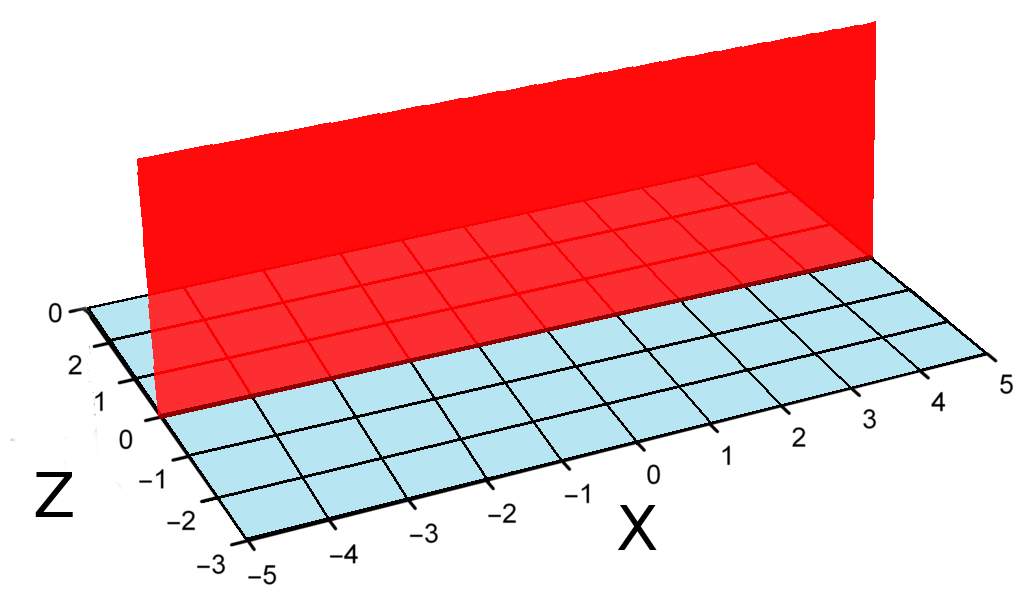
\includegraphics[scale=.7]{figures/GaussRel/squeezed.png}
%&\begin{matrix}\mapsto \\ \\ \\ \\ \end{matrix}
%&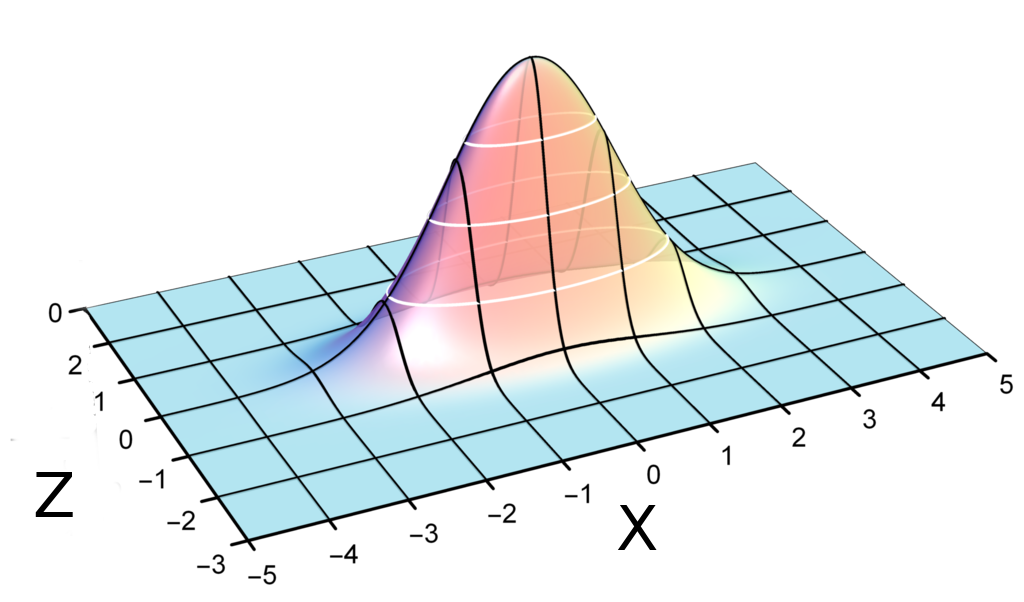
\includegraphics[scale=.7]{figures/GaussRel/coherent.png}\\
%?&&?\\
%\tikzfig{figures/GaussRel/vacuum_state}& \mapsto & \tikzfig{figures/GaussRel/vacuum_state}
%\end{array}
%\]


\hspace*{-.75cm}
\(
\displaystyle
\xymatrix@R+0pc@C+3.7pc{
\text{Dirac delta ``distribution''} & \text{Gaussian density function}\\
{\vcenteredincludenew{scripts/dirac_delta.png}} \ar@{|->}[r]^{\begin{matrix}\text{convolution by}\\ \mathcal{N}\left(\begin{bmatrix} \epsilon & 0\\ 0 & \epsilon^{\minu 1} \end{bmatrix}, \begin{bmatrix} 0 \\ 0 \end{bmatrix} \right) \end{matrix}} \ar@{<~>}[d]&
{\vcenteredincludenew{scripts/finitely_squeezed.png}}\ar@{<~>}[d] \\
\tikzfig{figures/GaussRel/infinitely_squeezed_state} \ar@{|->}[r]_{\tikzfig{figures/GaussRel/convolution_circuit}}&
\tikzfig{figures/GaussRel/squeezed_state}
}
\)

\end{frame}



\begin{frame}{Generators and equations for Gaussian QM}
Syntactically, adding the vacuum is  generated by freely codiscarding symplectic rotations \({\sf SO}(2n)\cap{\sf Sp}(2n)\) and effects in \(\ALR[\R]\).

\

That is for all \(a,b \in \R\), \(\theta, \vartheta \in [0,2\pi)\) with \(\vartheta\notin \{\pi/2,3\pi/2\}\):
\[\tikzfig{figures/GaussRel/axioms}\]
\end{frame}

\begin{frame}{Intuition for discarding}
The vacuum Gaussian on 1-qumode is the standard bivariate normal distribution:
\[
\xymatrix{
\tikzfig{figures/GaussRel/vacuum_state} \ \ \ar@{<~>}[rr]&&
\mbox{\!\!\!\!\!\!\!\vcenteredinclude{scripts/vacuum.png}}
}
\]


This is the only Wigner representation of a state which is invariant under rotation. 


\

Higher dimensions harder to visualize.
\end{frame}

\begin{frame}{Picturing quantum teleportation}
Following \cite{braunstein_teleportation_1998}:\\
Alice and Bob share a Gaussian Bell state with covariance of position $0<\varepsilon \in \R$.\\
Alice records the homodyne measurement outcome \((a,b)\in\R^2\) in the Bell basis, and sends it to Bob,\\ who performs the phase correction \({\hat p}^{- b} {\hat q}^{- a} \):
\[
\tikzfig{figures/GaussRel/teleportation_rotated}
\]
The result is a quantum channel with an error; however, in the infinitely-squeezed limit of \(\varepsilon=0\) there is no error.
%modified from 
%https://datasciencegenie.com/3d-contour-plots-of-bivariate-normal-distribution/
\end{frame}



\section{Research outlook: what remains to be done}



\begin{frame}{Conclusion}
We have turned the following Grassmanians into categories:

\emph{Affine Lagrangian/ coisotropic /positive Lagrangian}

\

And given generators and relations+quantum interpretations.


\

What is next?
\begin{itemize}
\item \textbf{Orthogonal Grassmanian:} \\
fermionic phase-space representation.

Lagrangian with respect to inner product.

\

\item \textbf{Twisted affine coisotropic Grassmaninan:} \\ Quantum dynamics \(\K((s))\)-affine subspaces.

Coisotropic with respect to Hermitian form \(\omega_{n,m}'(f(s), g(s)) \coloneqq \omega_{n,m}(f(s), g(1/s))\)

\end{itemize}

\end{frame}


\begin{frame}[allowframebreaks]
        \frametitle{References}
        \bibliography{styles/bibliography}
\end{frame}

\end{document}


